\section{Proposed dataset}

Three bright-field microscopy images datasets were acquired with the ZEISS Axiocam ERc5s camera in the ZEISS SteREO Discovery.v20 and the ZEISS AxioLab A1 stereo microscopes from the Scientific Computing Group (SCG) at São Carlos Institute of Physics (IFSC). The datasets contain images from leaf histological samples of the plants \textit{Callisia repens}, \textit{Tradescantia zebrina} and \textit{Cthenante oppenheimiana}, acquired with different focal planes and with different magnification levels. 

A shared feature among the species \textit{Callisia repens}, \textit{Tradescantia zebrina} and \textit{Cthenante oppenheimiana} is the purple abaxial (lower or bottom) leaf surface. This is commonly observed in deeply-shaded understorey plants and can be either transient or permanent, depending on the species and environmental conditions \cite{filho2018plants}. Several research projects have been conducted by the SCG group on plant leaf images, including biological studies with complex network analysis, where the locations of particular structures of the leaf, i.e. the stomata, were modeled as graphs. The \emph{stoma} (plural \emph{stomata}) is a structure that consists of an aperture between two cells, named \emph{guard cells}, and controls the exchange of steam, CO$_{2}$ and other gases from the inner part of the leaf and the atmosphere  \cite{hetherington2003role}. Furthermore, the concentration of stomata in leaves of purple plants is high; such stomatal cells are green and create a contrast between the epidermis and the stomata, which yields very good results with optical microscopy imaging \cite{filho2018plants}. Samples of blurred and sharp images of both datasets are shown in \autoref{fig:datasets}.

\begin{figure}[ht]
	\centering
	\caption{Examples of the proposed dataset images: blurred \textit{Callisia} \textbf{(a)}, sharp \textit{Callisia} \textbf{(b)}, blurred \textit{Tradescantia} \textbf{(c)}, sharp \textit{Tradescantia} \textbf{(d)} and blurred \textit{Cthenante} \textbf{(e)}, sharp \textit{Cthenante} \textbf{(f)}.}
	\label{fig:datasets}
	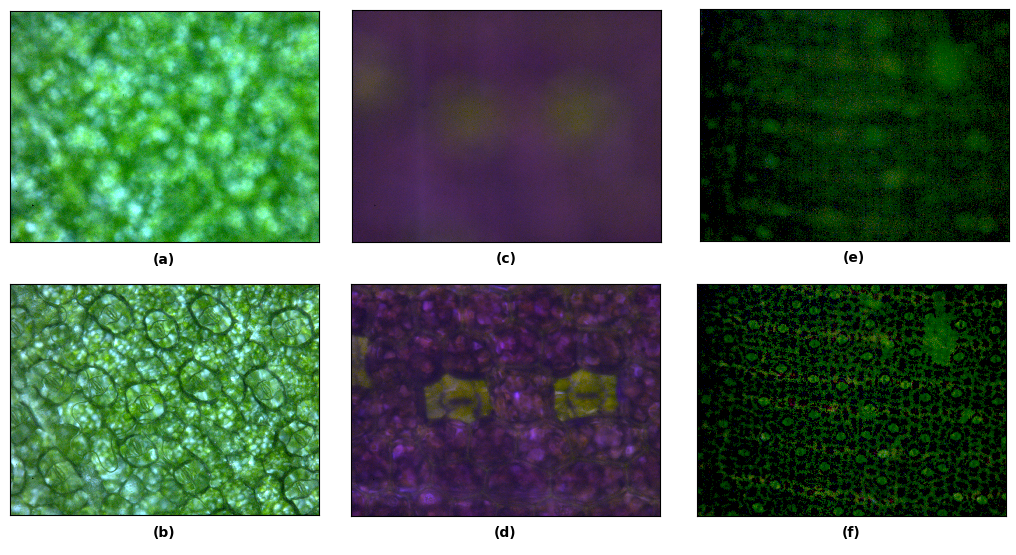
\includegraphics[scale=0.4]{images/datasets.png}
	\centering
	\fautor
\end{figure}

\subsection{Acquisition and Usage Protocols}

We will refer to the datasets as \textit{Callisia}, \textit{Tradescantia} and \textit{Cthenante} for notation simplicity. The \textit{Callisia} and \textit{Tradescantia} datasets were acquired with the z-stacking method in the SteREO Discovery.v20 microscope, whereas the \textit{Cthenante} dataset was acquired with the AxioLab A1 microscope. The workstation was connected to the microscopes by means of the ZEISS Axiovision version 4.8 software package. The z-stacks were manually built, i.e. the axial location of the objective was manually changed.

The SteREO Discovery.v20 microscope allows a precise measurement of the objective height, and the slices were acquired with a distance of 10 $\mu$m between each other - the maximum manually achievable distance. For both microscopes, the acquisition started with the objective height above the focal plane and, therefore, a completely blurred image. Then, the objective was progressively lowered in the $z$ axis, and at each step, an image was taken; this process was done until the objective height was below the focal plane and the images were blurred again.

The z-stacks were registered for image fusion after the eligible images in each set were chosen. Therefore, after the IQA method was applied, each set of eligible images was aligned with the TrakEM2 package, an ImageJ-based tool for processing and analyzing microscopy images. It includes methods for lens distortion correction, stitching, serial section alignment, correction of section thickness, and contrast adjustment \cite{saalfeld2019computational}. TrakEM2 uses  a particular combination of methods. The feature extraction was done with a custom implementation of the \sigla{SIFT}{Scale Invariant Feature Transform}, together with a custom extension of the \sigla{RANSAC}{Random Sample Consensus} method for parameter estimation and the geometric consensus filtering process with the expected transformation model and a maximal expected error as parameters \cite{saalfeld2019computational}. 

Primarily, a subjective quality index based on the Mean Opinion Score (MOS) was built in order to validate the results. The mean opinion score is the average of values on a predefined scale that an observer assigns to his opinion about the performance of a system (in this case, the imaging system) across a sample of observers \cite{liu2019comprehensive}. Practically, it consists of integer numbers in the interval $[1,5]$ where 1 is the worst score and 5 is the best. With the output of three people - two microscopy experts and one from a non-microscopy field - a subjective index was created. Most of the images were classified as 1 and the maximum score was 3. The images were then labeled as 3 - \emph{eligible} and 1 or 2 - \emph{negligible} for the fusion process, respectively. The axial nature of the acquisition allowed for a contiguous set of eligible images in each dataset. \autoref{tab:dataset_info} presents some relevant properties of each dataset.

\begin{table}[ht]
    \centering
    \caption{Information about the proposed datasets.}
    \label{tab:dataset_info}
    \begin{tabular}{lccc}
        \toprule
        \textbf{Dataset} & \textbf{\textit{Callisia}} &
        \textbf{\textit{Tradescantia}} &
        \textbf{\textit{Cthenante}}\\
        \midrule
        \textit{Magnification} & 50x & 200x & 100x\\
        \textit{Step} & 10$\mu$m & 10$\mu$m & 4$\mu$m\\
        \textit{Number of images} & 56 & 66 & 55\\
        \textit{Eligible} & 9 & 2 & 16\\
        \textit{Sharp sequence} & 41 - 49 & 50 - 51 & 30 - 45\\
        \bottomrule
    \end{tabular}
    \centering
    \fautor
\end{table}

In order to use the proposed datasets for evaluation of new methods, it is necessary to take into account that several images are totally blurred, and an image quality assessment algorithm should yield a low metric number for such images. As the $z$ position approaches the optimal focal plane, the metric may start to produce better values. The images are named with the step of the $z$-stack starting at 1, so that the eligible images are easily located. The metric should yield the highest quality values are among the range of eligible images, depicted as 
``Sharp sequence'' in \autoref{tab:dataset_info}. When the axial position is not exceeds the limits of the sharp sequence, the metric values should decay. The datasets are capable of assessing the monotonicity, accuracy and precision of image quality metrics.

\section{Benchmark datasets}

Benchmark datasets are fundamental in computer vision and image processing research in order to track the performance, accuracy and efficiency of new methods and algorithms. The image quality assessment was also evaluated against literature methods with the well-known Computational and Subjective Image Quality database (CSIQ) image quality assessment database \cite{larson2010most} and the KonIQ database, the largest image quality assessment database to date \cite{hosu2020koniq}. 

The CSIQ database contains 30 original images of dimensions $512 \times 512$. Each image is distorted in four to five different levels separately by JPEG and JPEG-2000 compression, Gaussian blurring, global contrast decrements and additive pink Gaussian noise. The Gaussian blur subset with 150 images was employed in the proposed analysis. The dataset also contains 5000 subjective rates done by 35 different observers, By means of a MOS index. 

The KonIQ database was built in order to evaluate the performance of a deep learning method for blind image quality assessment. It consists of 10073 images of dimensions $1024 \times 768$ with different labels for brightness, contrast, colorfulness and sharpness. The labels were generated from 1.2 million MOS rating of 1459 observers. One dissimilar feature of KonIQ when compared to CSIQ is that the quality assessment should be done among different scenes with different levels of degradation. \autoref{fig:csiq_example} shows two samples of the CSIQ database, and \autoref{fig:koniq_example} presents both blurred and sharp samples from the KonIQ image.

\begin{figure}[htb]
    \centering
    \caption{Samples from the CSIQ database: blurred image (a) and sharp image (b).}
    \label{fig:csiq_example}
    \begin{subfigure}[t]{0.45\textwidth}
        \centering
        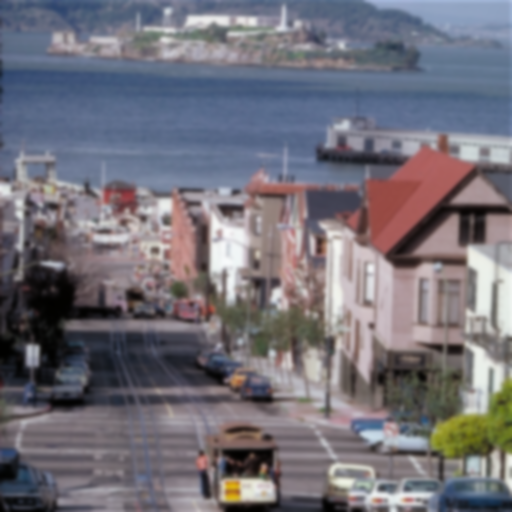
\includegraphics[height=5cm]{images/csiq_blurred.png}
        \caption{}
    \end{subfigure}%
    ~ 
    \begin{subfigure}[t]{0.5\textwidth}
        \centering
        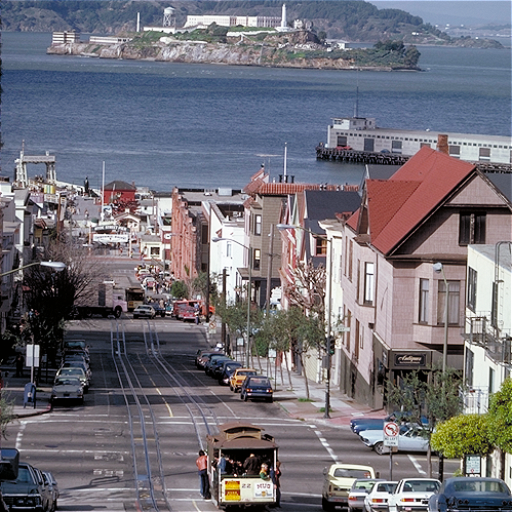
\includegraphics[height=5cm]{images/csiq_sharp.png}
        \caption{}
    \end{subfigure}
    \centering
    \fdireta{larson2010most}
\end{figure}

\begin{figure}[htb]
    \centering
    \caption{Samples from the KonIQ database: blurred image (a) and sharp image (b).}
    \label{fig:koniq_example}
    \begin{subfigure}[t]{0.45\textwidth}
        \centering
        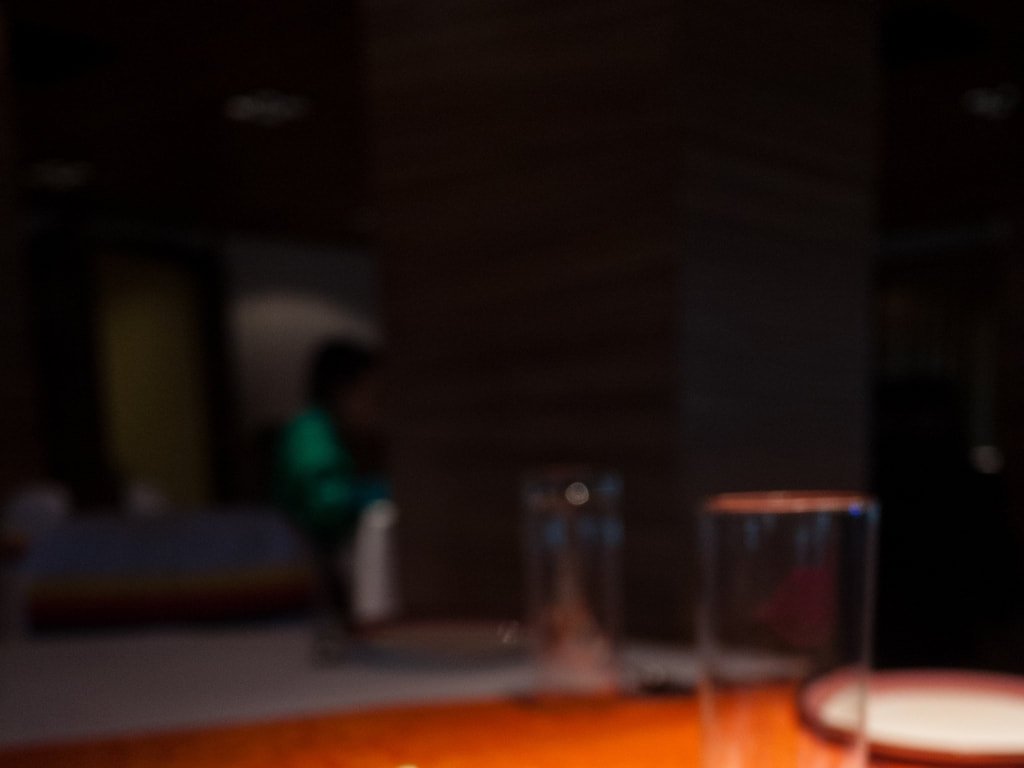
\includegraphics[height=4cm]{images/koniq-blurred.jpg}
        \caption{}
    \end{subfigure}%
    ~ 
    \begin{subfigure}[t]{0.45\textwidth}
        \centering
        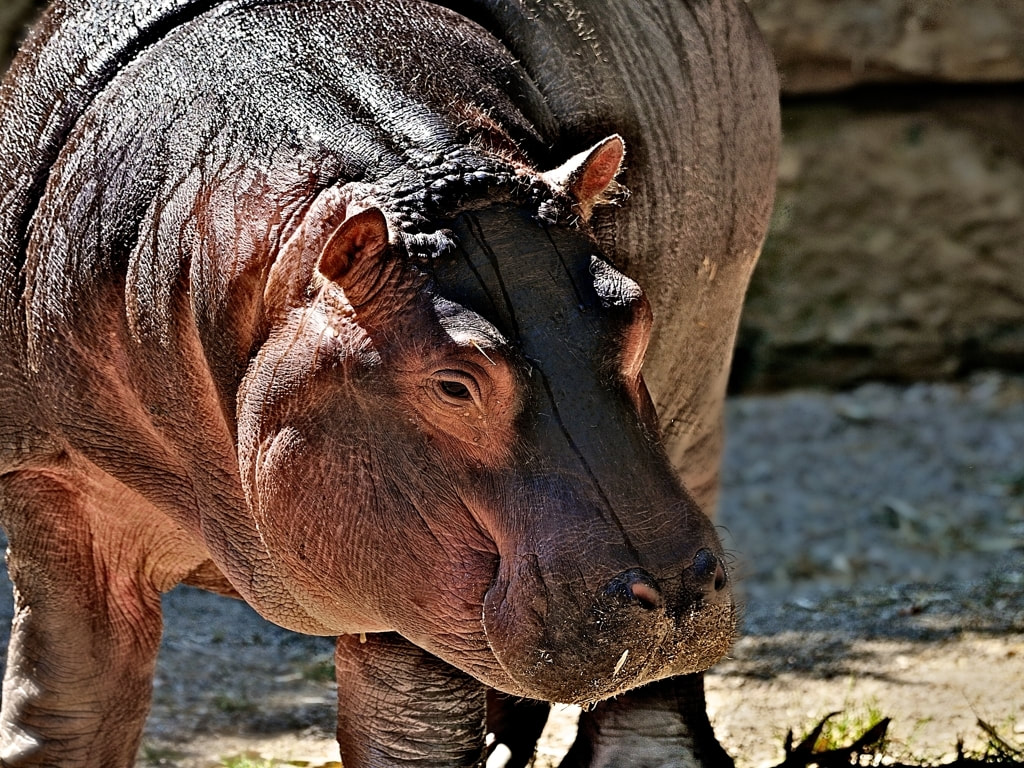
\includegraphics[height=4cm]{images/koniq-sharp.jpg}
        \caption{}
    \end{subfigure}
    \centering
    \fdireta{hosu2020koniq}
\end{figure}